\documentclass{article}
\setlength{\parindent}{0cm}

@(vfl) = **Vanilla Flavored LaTex**

@(github_url) = http://github.com/adhithyan15/vanilla

@(tmaker) = **TexMaker**

@(ftb) = formatted text blocks

$(importpack)[documentation]

\begin{document}

\begin{center}

\huge{Vanilla Documentation}\vspace{5pt}

\large{**Adhithya Rajasekaran**}

\end{center}

\vspace{30pt}

\section*{What is Vanilla?}

Vanilla is a powerful LaTex preprocessor. It aims to reduce the entry barrier and learning curve for Latex by simplifying the syntax and also reducing the verbosity of Latex. In this documentation you will learn how to write Vanilla flavoured Latex documents. This document itself is written in Vanilla flavoured Latex. \vspace{5pt}

Let us start off with why I created Vanilla. \vspace{5pt}

\section*{Why Vanilla?}

I was trying to teach my mom, who is a high school math teacher, to use Latex. I was unsuccessful in that endeavour because my mom found Latex syntax very verbose and she hated the steep learning curve of Latex. I started to wonder if there are any ways to reduce the learning curve of Latex and also reduce the verbosity of Latex. I stumbled across \textbf{Markdown}, a small markup language that compiled into HTML. The syntax of Markdown was very intuitive and short. So I decided to implement a lot of ideas from Markdown into Latex and that's how Vanilla was born. 

\section*{Technical Details}

Vanilla first started out as a separate markup language with backward compatiblity to Latex. But I dropped that idea and made it as an extension of Latex so that people can keep using their editors. Vanilla compiler prototype was written in Python. Then the code was translated into Ruby and was released as a command line utility.

\section*{Getting Vanilla}

It is very easy to get Vanilla. Visit www.adhithyan15.github.com/vanilla/ and follow the steps below. 

#(list)
1. Click on ``Download Zip'' to download both the source of the compiler and also the compiled version of the compiler. \vspace{5pt}

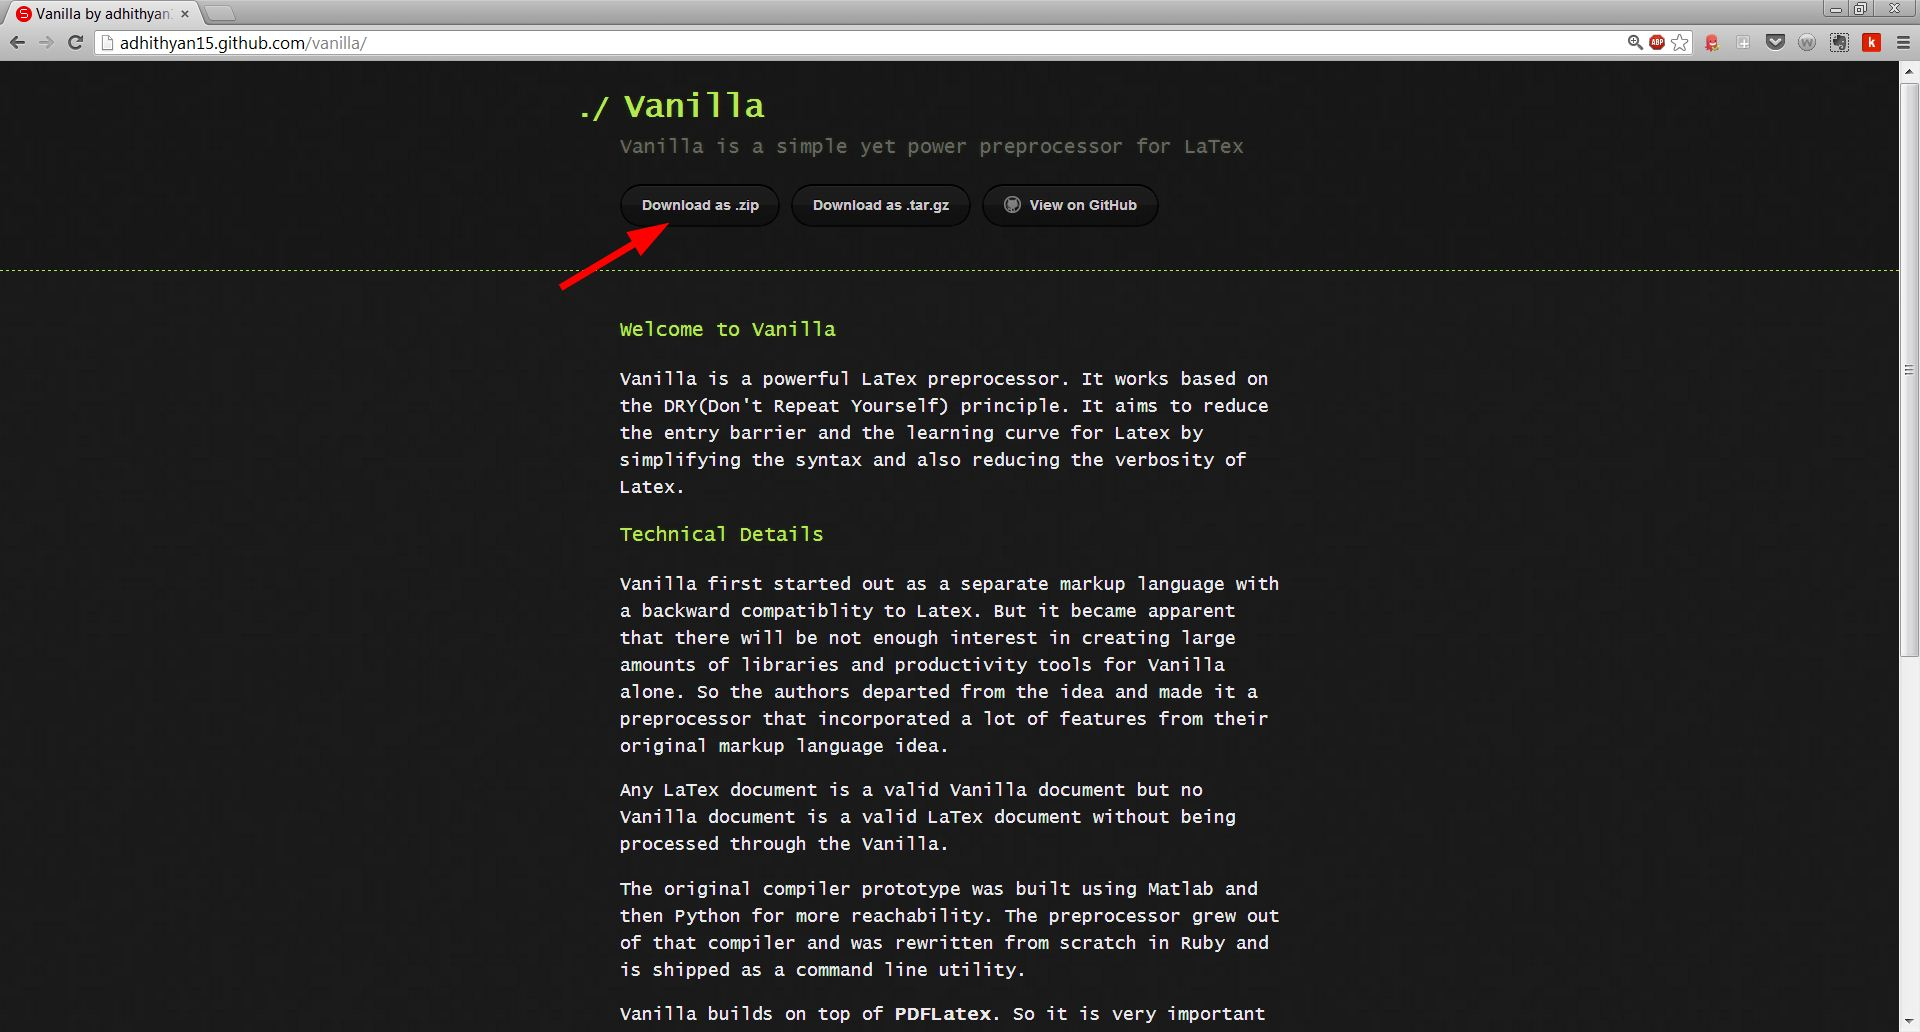
\includegraphics[scale=0.5]{VanillaGithub}

2. Extract the downloaded zip file using Winzip or any other archive extractor. If you don't have an archive extractor, I recommend *[ 7-zip => www.7zip.org ]

3. Once you extract it, you will find the following files inside the folder you extracted

#(nlist)

* Vanilla.exe  -> This is the primary compiler that will help you compile @(vfl) to **Pure LaTex**. This might be of no use to you if you are running linux or mac. 
* Vanilla.rb  ->  This file contains the source code of the compiler. If you are in mac or linux, you can use this file to compile your **Vanilla Flavored LaTex** to LaTex documents.
* Readme.md ->  Since the project is hosted in *[ Github => @(github_url) ], Github added a readme file markuped in **Markdown**.
* Documentation.pdf ->  This is the same document that you are reading right now. 
* Documentation.tex ->  This is the .tex version of documentation written using @(vfl). I highly recommend you to read through this document so that you can get example usages of @(vfl). 

#(endnlist)

%{4. If you don't have a LaTex editor, I highly recommend *[ TexMaker => http://www.xm1math.net/texmaker/]. It is the best LaTex editor that I was able to find. In the next section, we will learn how to configure **TexMaker** to use @(vfl).}%
 
#(endlist)

Vanilla compiler can work with LaTex Editors. But I request you to not use it because there are some issues which are being worked out. I expect to resolve all the issues by Version 2.0. So please wait until such time.

\section*{Features of Vanilla}

@(vfl) offers a lot of features to enhance people's productivity with LaTex. Let us see what those features below

#(list)

* Multiline Comments -> LaTex does offer multiline comments through the **Verbatim** package and there is also a way to comment out multiple lines of code using **iffalse** command.
In @(vfl) you can comment out multiple lines of code using matlab style comments. Let us see a quick demo of this feature

###
%LaTex Way

\usepackage{verbatim} %In the preamble

\begin{comment} %In the body

Lorem ipsum dolor sit amet, consectetur adipiscing elit. Mauris placerat tristique purus, 
non tempus mi ultrices in. Praesent lobortis erat et lorem commodo mollis. Pellentesque eu 
euismod nulla. Ut vitae consequat est. Quisque adipiscing rhoncus tellus, eu fermentum 
augue tincidunt ut. Proin a dui dignissim massa auctor iaculis dictum a purus. 
Suspendisse porta felis at velit placerat varius.

\end{comment}

%Vanilla Way

%You can comment out multiple lines using matlab style comments %{.....}%

%{Lorem ipsum dolor sit amet, consectetur adipiscing elit. Mauris placerat tristique purus, 
non tempus mi ultrices in. Praesent lobortis erat et lorem commodo mollis. Pellentesque 
eu euismod nulla.Ut vitae consequat est. Quisque adipiscing rhoncus tellus, eu fermentum 
augue tincidunt ut. Proin a dui dignissim massa auctor iaculis dictum a purus. Suspendisse 
porta felis at velit placerat varius.}%

###

Vanilla compiler converts @(vfl) multiline comments into several single line LaTex comments. Vanilla compiler doesn't touch the LaTex comments. So they are still valid. 

* Constants -> Constants are very similar to variables but they are immutable. LaTex does offer constants through **newcommand** option. In @(vfl), you can declare constants
through the following sytax $@(constant\_name) = value$. Note: LaTex has offers mutable variables. We are working on implementing mutable variables in Vanilla. It will be released in
version 2.0. 

###

%LaTex way

\newcommand{\vfl}{\textbf{Vanilla Flavored LaTex}} %can be declared anywhere in the body

%Usage

Welcome to \vfl %Welcome to \textbf{Vanilla Flavored LaTex}

%Vanilla way

%Vanilla forces you to declare your constants in your preamble so that it will 
%increase code readability. 

@(vfl) = **Vanilla Flavored LaTex** %must be declared in the preamble

%Usage

Welcome to @(vfl) %should output Welcome to \textbf{Vanilla Flavored LaTex} 

%LaTex Mutability

%You can modify the variable \vfl using the \renewcommand

\renewcommand{\vfl}{\textbf{Vanilla}} %can be done anywhere on the body

%Usage

Welcome to @(vfl) %should output Welcome to \textbf{Vanilla} 

###

* Formatted Text Blocks -> Formatted Text Blocks were inspired by Less CSS' parametric mixins.
@(vfl) forces the @(ftb) to be declared inside preamble to increase readability and @(ftb) are immutable. You can de But
I am working on working on creating a mutable version of @(ftb) and it will be released in version 2.0. LaTex does offer
support for something similar to @(ftb) using the **\\newcommand** and they are mutable through **\\renewcommand**. Let us see a quick demo of this
feature

###

%LaTex way

\newcommand

### 

#(endlist)

\end{document}